% -*- TeX -*-
\documentclass[aspectratio=169]{beamer}

\title{PyLith v4.1 Tutorial}
\subtitle{Meshing with Gmsh: Multiple faults in 2D and 3D}
\author{Brad Aagaard\\
  Charles Williams \\
  Matthew Knepley}
\institute{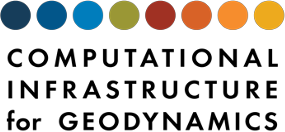
\includegraphics[scale=1.5]{../../logos/cig_logo_dots}%
  \hspace{4em}%
\raisebox{1em}{\includegraphics[scale=1.0]{../../logos/cig_short_pylith}}}
\date{June 11, 2024}


% ---------------------------------------------------- CUSTOMIZATION
\usetheme{CIG}
% Style information for PyLith presentations.

% Colors
\definecolor{ltorange}{rgb}{1.0, 0.74, 0.41} % 255/188/105
\definecolor{orange}{rgb}{0.96, 0.50, 0.0} % 246/127/0

\definecolor{ltred}{rgb}{1.0, 0.25, 0.25} % 255/64/64
\definecolor{red}{rgb}{0.79, 0.00, 0.01} % 201/0/3

\definecolor{ltpurple}{rgb}{0.81, 0.57, 1.00} % 206/145/255
\definecolor{purple}{rgb}{0.38, 0.00, 0.68} % 97/1/175

\definecolor{ltblue}{rgb}{0.2, 0.73, 1.0} % 51/187/255
\definecolor{mdblue}{rgb}{0.28, 0.50, 0.80} % 72/128/205
\definecolor{blue}{rgb}{0.12, 0.43, 0.59} % 30/110/150

\definecolor{ltltgreen}{rgb}{0.7, 1.00, 0.7} % 96/204/14
\definecolor{ltgreen}{rgb}{0.37, 0.80, 0.05} % 96/204/14
\definecolor{green}{rgb}{0.23, 0.49, 0.03} % 59/125/8
  
\definecolor{dkslate}{rgb}{0.18, 0.21, 0.28} % 47/53/72
\definecolor{mdslate}{rgb}{0.45, 0.50, 0.68} % 114/127/173
\definecolor{ltslate}{rgb}{0.85, 0.88, 0.95} % 216/225/229


\newcommand{\includefigure}[2][]{{\centering\includegraphics[#1]{#2}\par}}
\newcommand{\highlight}[1]{{\bf\usebeamercolor[fg]{structure}#1}}
\newcommand{\important}[1]{{\color{red}#1}}
\newcommand{\issue}[2]{\item[Issue:] {\color{red}#1}\\{\item[Soln:] \color{blue}#2}\\[4pt]}

\setbeamercolor{alerted text}{fg=ltgreen}
\setbeamertemplate{description item}[align left]


\newcommand{\lhs}[1]{{\color{blue}#1}}
\newcommand{\rhs}[1]{{\color{red}#1}}
\newcommand{\annotateL}[2]{%
  {\color{blue}\underbrace{\color{blue}#1}_{\color{blue}\mathclap{#2}}}}
\newcommand{\annotateR}[2]{%
  {\color{red}\underbrace{\color{red}#1}_{\color{red}\mathclap{#2}}}}
\newcommand{\eqnannotate}[2]{%
  {\color{blue}%
  \underbrace{\color{black}#1}_{\color{blue}\mathclap{#2}}}}

\newcommand{\trialvec}[1][]{{\vec{\psi}_\mathit{trial}^{#1}}}
\newcommand{\trialscalar}[1][]{{\psi_\mathit{trial}^{#1}}}
\newcommand{\basisvec}[1][]{{\vec{\psi}_\mathit{basis}^{#1}}}
\newcommand{\basisscalar}[1][]{{\psi_\mathit{basis}^{#1}}}

\newcommand{\tensor}[1]{\bm{#1}}
\DeclareMathOperator{\Tr}{Tr}

\usefonttheme[onlymath]{serif}

% minted shortcuts
\newminted{cfg}{bgcolor=ltslate,autogobble,fontsize=\tiny}
\newminted{bash}{bgcolor=ltltgreen,autogobble,fontsize=\tiny}

% PyLith components
\newcommand{\pylith}[1]{{\ttfamily\color{magenta}#1}}



% --------------------------------------------------------- DOCUMENT
\begin{document}

% ------------------------------------------------------------ SLIDE
\maketitle

\logo{\includegraphics[height=4.5ex]{../../logos/cig_short_pylith}}

% ========================================================== SECTION
\section{Overview}
\subsection{Workflow and Tips}

% ------------------------------------------------------------ SLIDE
\begin{frame}[t]
  \frametitle{Gmsh and Cubit Workflow}
  \summary{}

  \begin{enumerate}
  \item Create geometry
    \begin{onlyenv}<1>
      \begin{enumerate}
      \item Construct surfaces from points, curves, etc or basic shapes
      \item Create domain and subdivide to create any interior surfaces
        \begin{itemize}
        \item Fault surfaces must be interior surfaces
        \item Need separate volumes for different constitutive {\em models, not parameters}
        \end{itemize}
      \end{enumerate}
    \end{onlyenv}
  \item Tag entities\\
    Gmsh: Tag {\em before} generating mesh. Cubit: Tag {\em after} generating mesh
    \begin{onlyenv}<2>
      \begin{enumerate}
      \item Tag surfaces (2D domain) or volumes (3D domain) for each material
      \item Tag entities for each boundary condition or fault
        \hitem{Tag entities for buried fault edges}
      \item Tag ground surface for output (optional)
      \end{enumerate}
    \end{onlyenv}
  \item Create finite-element mesh
    \begin{onlyenv}<3>
      \begin{enumerate}
      \item Specify meshing scheme
      \item Specify mesh sizing information
      \item Generate mesh
      \item Smooth to fix any poor quality cells
      \end{enumerate}
    \end{onlyenv}
  \item Write mesh to file\only<4>{}
  \end{enumerate}

\end{frame}


% ------------------------------------------------------------ SLIDE
\begin{frame}
  \frametitle{Mesh Generation Tips}
  \summary{Keep in mind the scales of the observations you are modeling}

  \begin{itemize}
  \hitem{Topography/bathymetry}
    \begin{itemize}
    \item Ignore topography/bathymetry unless you know it matters
    \end{itemize}\pause
  \hitem{Fault surfaces}
    \begin{itemize}
    \item Building surfaces from contours is usually easiest
    \item Include features at the resolution that matters
    \end{itemize}\pause
  \hitem{Performance}
    \begin{itemize}
    \item Number of points in spline curves/surfaces often has huge effect on mesh generation runtime
    \item Use uniform refinement in PyLith whenever possible
    \item Use basis order of 2 or 3 to get same or better accuracy with larger cells
    \end{itemize}
  \end{itemize}

\end{frame}


% ------------------------------------------------------------ SLIDE
\begin{frame}
  \frametitle{Mesh Generation Tips (cont.)}
  \summary{There is no silver bullet in finite-element mesh generation}
 
  \begin{itemize}
  \hitem{Hex/Quad versus Tet/Tri}
    \begin{itemize}
    \item Hex/Quad are slightly more accurate and faster
    \item Tet/Tri easily handle complex geometry
    \item Easy to vary discretization size with Tet, Tri, and Quad cells
    \item There is no easy answer\\
      For a given accuracy, a finer resolution Tet mesh that varies
      the discretization size in a more optimal way {\bf\it might} run
      faster than a Hex mesh
    \end{itemize}\pause
  \hitem{Check and double-check your mesh}
    \begin{itemize}
    \item Were there any errors when running the mesh generator?
    \item Are the boundaries, etc marked correctly?
    \item Check mesh quality (aspect ratio should be close to 1)
    \end{itemize}
  \end{itemize}

\end{frame}


% ------------------------------------------------------------ SLIDE
\begin{frame}
  \frametitle{Mesh Generation Tips  (cont.)}
  \summary{}

  \begin{description}
    \issue{Changes in geometry cause changes in object ids} {Name objects and use
      variables to eliminate hardwired ids wherever possible}\pause
    \issue{Splines with many points slow down operations}{Minimize the
      number of points per spline}\pause
    \issue{Surfaces meet in small angles creating distorted
      cells}{Trim geometry to eliminate features smaller than cell
      size}\pause
    \issue{Difficulty meshing complex geometry with hexahedral or quadrilateral cells}{Use
      tetrahedral or triangular cells even if it requires a finer mesh}\pause
    \issue{Hexahedral mesh over-samples parts of the
      domain}{Use tetrahedral mesh and vary discretization within domain}\pause
    \issue{Extended surfaces create very complex geometry}{Embed
      surfaces to eliminate overly complex geometry}
  \end{description}

\end{frame}


% ========================================================== SECTION
\section{{\ttfamily examples/crustal-strikeslip-2d}}
\subsection{Workflow}

% ------------------------------------------------------------ SLIDE
\begin{frame}
  \frametitle{Intersecting strike-slip faults in 2D}
  \summary{{\ttfamily examples/crustal-strikeslip-2d}}

  \includefigure[height=7.0cm]{figs/geometry2d}
  
\end{frame}


% ------------------------------------------------------------ SLIDE
\begin{frame}
  \frametitle{Creating the finite-element mesh with Gmsh}
  \summary{}

  We construct the geometry by first creating points, then connecting the points into curves, and finally the curves into surfaces using the Gmsh geometry engine.
  
  \includefigure[height=6.5cm]{figs/geometry2d-gmsh}
  
\end{frame}


% ------------------------------------------------------------ SLIDE
\begin{frame}
  \frametitle{Setting up the model}
  \summary{}
  
  \begin{enumerate}
  \item Prepare fault traces
    \begin{enumerate}
    \item Choose appropriate resolution of fault trace information
    \item Choose geographic projection for georeferencing (UTM 11N, {\ttfamily EPSG:32611})
    \item Convert fault traces (latitude and longitude, {\ttfamily EPSG:4326}) to UTM 11N using {\ttfamily cs2cs}
    \item Ensure fault traces have common point(s) at intersections
    \end{enumerate}\pause
  \item Choose dimensions of domain (80 km x 80 km)\\
    Edge of domain is several rupture dimensions from the faults
  \end{enumerate}
  
\end{frame}


% ------------------------------------------------------------ SLIDE
\begin{frame}
  \frametitle{Gmsh: Creating the geometry}
  \summary{}
  
  \begin{enumerate}
  \item Create domain\\
    points $\rightarrow$ curves $\rightarrow$ curve loop $\rightarrow$ surface\pause
  \item Create fault traces
    \begin{enumerate}
    \item Read fault traces from file using {\ttfamily numpy.loadtxt}
    \item points $\rightarrow$ spline
    \end{enumerate}\pause
  \item Clean up: remove duplicate points at fault intersection(s)\pause
  \item Embed fault curves (dim=1) in domain surface (dim=2) using {\ttfamily embed}
  \end{enumerate}
  
\end{frame}


% ------------------------------------------------------------ SLIDE
\begin{frame}
  \frametitle{Gmsh: Creating the mesh}
  \summary{Same process as simple mesh with a little more emphasis on cell size parameters}
  
  \begin{enumerate}
  \item Mark boundaries, interfaces, and materials\pause
  \item Generate the mesh\pause
    \begin{enumerate}
    \item Choose cell size on faults
      \begin{itemize}
      \item Region with highest strain gradients $\rightarrow$ smallest cell size
      \item Small enough size to resolve geometry and slip distribution
      \item We can refine and use higher order discretization to increase resolution
      \end{itemize}\pause
    \item Create field with distance from faults\pause
    \item Create field with cell size based on distance from faults
      \begin{itemize}
      \item Choose gradient for increasing cell size away from faults (typically 1.05-1.10)
      \item Resolve spatial variations in displacement or strain
      \end{itemize}\pause
    \item Generate mesh using cell size field
    \end{enumerate}\pause
  \item Apply Laplacian smoothing to improve mesh quality
  \end{enumerate}
  
\end{frame}


\subsection{Final Mesh}

% ------------------------------------------------------------ SLIDE
\begin{frame}
  \frametitle{Gmsh: Finite-Element Mesh}
  \summary{{\ttfamily ./generate\_gmsh.py --write --gui}}

  \includefigure[height=7.0cm]{figs/gmsh-tri}
  
\end{frame}


% ========================================================== SECTION
\section{{\ttfamily examples/crustal-strikeslip-3d}}
\subsection{Workflow}

% ------------------------------------------------------------ SLIDE
\begin{frame}
  \frametitle{Intersecting strike-slip faults in 3D}
  \summary{{\ttfamily examples/crustal-strikeslip-3d}}

  \includefigure[height=7.0cm]{figs/geometry3d}
  
\end{frame}


% ------------------------------------------------------------ SLIDE
\begin{frame}
  \frametitle{Creating the finite-element mesh with Gmsh}
  \summary{}

  We use the \href{https://dev.opencascade.org/}{Open Cascade} geometry engine to create solid geometry.
  
  \includefigure[height=6.5cm]{figs/geometry3d-gmsh}
  
\end{frame}


% ------------------------------------------------------------ SLIDE
\begin{frame}
  \frametitle{Setting up the model}
  \summary{}
  
  \begin{enumerate}
  \item Prepare fault traces (same as 2D)
  \item Choose how to extend surface traces to depth (we assume vertical faults)
  \item Choose dimensions of domain (80 km x 60 km x 40 km)
    \begin{itemize}
    \item Edge of domain is several rupture dimensions from the faults
    \item Avoid small cell sizes or distorted cells at interfaces and boundaries
    \end{itemize}
  \end{enumerate}
  
\end{frame}


% ------------------------------------------------------------ SLIDE
\begin{frame}
  \frametitle{Gmsh: Creating the geometry}
  \summary{}
  
  \begin{enumerate}
  \item Create domain (box)\pause
  \item Create fault traces
    \begin{enumerate}
    \item Read fault traces from file using {\ttfamily numpy.loadtxt}
    \item points $\rightarrow$ spline
    \item Extrude curves to form surfaces using {\ttfamily extrude}
    \end{enumerate}\pause
  \item Embed fault surfaces (dim=2) in domain surface (dim=3) using {\ttfamily fragment}\pause
  \item Identify geometry entities using GUI
  \end{enumerate}
  
\end{frame}


% ------------------------------------------------------------ SLIDE
\begin{frame}
  \frametitle{Gmsh: Creating the mesh}
  \summary{Same process as simple mesh with a little more emphasis on cell size parameters}
  
  \begin{enumerate}
  \item Mark boundaries, interfaces, and materials
  \item Generate the mesh (same as 2D)
  \item Apply Laplacian smoothing to improve mesh quality
  \item Examine mesh along fault trace to check for any issues
    \begin{itemize}
    \item Cells should align with fault surface
    \item Cells edges should not cross intersections
    \end{itemize}
  \end{enumerate}
  
\end{frame}


\subsection{Final Mesh}

% ------------------------------------------------------------ SLIDE
\begin{frame}
  \frametitle{Gmsh: Finite-Element Mesh}
  \summary{{\ttfamily ./generate\_gmsh.py --write --gui}}

  \includefigure[height=7.0cm]{figs/gmsh-tet}
  
\end{frame}


% ------------------------------------------------------------ SLIDE
\begin{frame}
  \frametitle{Bonus Content: Including Topography}
  \summary{}

  \begin{itemize}
    \hitem{Resources}
    \begin{itemize}
      \item \href{https://www.usgs.gov/centers/eros/science/usgs-eros-archive-digital-elevation-global-multi-resolution-terrain-elevation}{Digital Elevation -- Global Multi-resolution Terrain Elevation Data 2010 (GMTED2010)}
    \item \href{https://earthexplorer.usgs.gov/}{Earth Explorer -- USGS} for browsing and downloading data
    \item \href{https://gdal.org}{GDAL} is a translator library for raster and vector geospatial data formats
    \item \href{https://docs.scipy.org/doc/scipy/reference/generated/scipy.spatial.Delaunay.html}{scipy.spatial.Delaunay} for creating triangulations of DEM data
    \item \href{https://numpy-stl.readthedocs.io/en/latest/usage.html}{numpy-stl} for creating STL files from triangulations
    \end{itemize}\pause
    \hitem{General workflow}
    \begin{enumerate}
    \item Download elevation data (Earth Explorer)
    \item Extract subset at desired resolution ({\ttfamily gdal\_translate})
    \item Create surface
    \item Build geometry using surface
    \item Generate finite-element mesh for geometry
    \end{enumerate}
  \end{itemize}

\end{frame}


% ------------------------------------------------------------ SLIDE
\begin{frame}
  \frametitle{Workflow \#1: Gmsh geometry engine}
  \summary{\href{https://gitlab.onelab.info/gmsh/gmsh/blob/master/examples/api/terrain_stl.py}{Gmsh example: terrain\_stl.py}}

  \begin{enumerate}
    \hitem{Download elevation model -- Earth Explorer}
    \begin{onlyenv}<1>
      \begin{enumerate}
      \item Select region
      \item Select dataset
      \item Download
      \item Extract file
      \end{enumerate}
    \end{onlyenv}
    \hitem{Extract subset at desired resolution -- {\ttfamily gdal\_translate} CLI or {\ttfamily gdal.Translate()} Python API}
    \begin{onlyenv}<2>
      \begin{enumerate}
      \item Set model region
      \item Set desired resolution
      \item Set output format
      \end{enumerate}
    \end{onlyenv}
    \hitem{Create STL file via Python script}
    \begin{onlyenv}<3>
      \begin{enumerate}
      \item Read in elevation data for model region -- {\ttfamily netCDF4}
      \item Transform to model coordinate system -- {\ttfamily spatialdata + proj} or {\ttfamily pyproj}
      \item Create triangulation -- {\ttfamily scipy.spatial.Delaunay}
      \item Create STL representation -- {\ttfamily numpy-stl}
      \end{enumerate}
    \end{onlyenv}
    \hitem{Create geometry in Gmsh}
    \begin{onlyenv}<4>
      \begin{enumerate}
      \item Load STL surface into Gmsh -- {\ttfamily gmsh.merge()}
      \item Create geometry from STL surface -- {\ttfamily gmsh.model.mesh.classifySurfaces()} and {\ttfamily gmsh.model.mesh.createGeometry()}
      \item Identify ids of points and curves -- GUI
      \item Create points, curves, and surfaces to create volume
      \end{enumerate}
    \end{onlyenv}
  \end{enumerate}

\end{frame}


% ------------------------------------------------------------ SLIDE
\begin{frame}
  \frametitle{Workflow \#2: Gmsh Open Cascade engine}
  \summary{\href{https://gitlab.onelab.info/gmsh/gmsh/blob/master/examples/api/terrain_bspline.py}{Gmsh example: terrain\_bspline.py}}

  \begin{enumerate}
    \hitem{Download elevation model -- Earth Explorer}
    \begin{onlyenv}<1>
      \begin{enumerate}
      \item Select region
      \item Select dataset
      \item Download
      \item Extract file
      \end{enumerate}
    \end{onlyenv}
    \hitem{Extract subset at desired resolution -- {\ttfamily gdal\_translate} CLI or {\ttfamily gdal.Translate()} Python API}
    \begin{onlyenv}<2>
      \begin{enumerate}
      \item Set model region
      \item Set desired resolution
      \item Set output format
      \end{enumerate}
    \end{onlyenv}
    \hitem{Create geometry in Gmsh}
    \begin{onlyenv}<3>
      \begin{enumerate}
      \item Read in elevation data for model region -- {\ttfamily netCDF4}
      \item Transform to model coordinate system -- {\ttfamily spatialdata + proj} or {\ttfamily pyproj}
      \item Add points -- {\ttfamily gmsh.model.occ.add\_point()}
      \item Create BSpline surface from points -- {\ttfamily gmsh.model.occ.add\_bspline\_surface()}
      \item Delete points -- {\ttfamily gmsh.model.occ.remove()}
      \item Create box (extending above topography) -- {\ttfamily gmsh.model.occ.add\_box()}
      \item Cut box with topgraphy -- {\ttfamily gmsh.model.occ.fragment()}
      \item Remove portion of box above topography -- {\ttfamily gmsh.model.occ.remove()}
      \end{enumerate}
    \end{onlyenv}
  \end{enumerate}

\end{frame}




% ======================================================================
\end{document}


% End of file
